\section{Global approach}
\label{tech:generic}

The work of Hilbig et al. \cite{Hilbig2021AnES} at 2021 influences our design decisions. According to their work, 70\% of the \wasm binaries in the wild are created with LLVM-based compilers. Therefore, we decided to provide Artificial Sotfware Diversity for \wasm through LLVM. 
Other solutions would have been to diversify at the source code level, or at the \wasm binary level. However, the former would limit the applicability of our work. The latter, is proposed for future works.

LLVM is compound of three main components \cite{llvmofficialweb}. First, the frontend (compilers such as clang and rustc) converts the program source code to LLVM intermediate representation (LLVM IR). Second, optimization and transformation passes improve the LLVM IR. Third and final, the backend component is in charge of generating the target machine code. In \autoref{diagrams:generic} we show how we use the LLVM pipeline in our contributions, which are highlighted as dashed squares.

\begin{figure*}[h]
    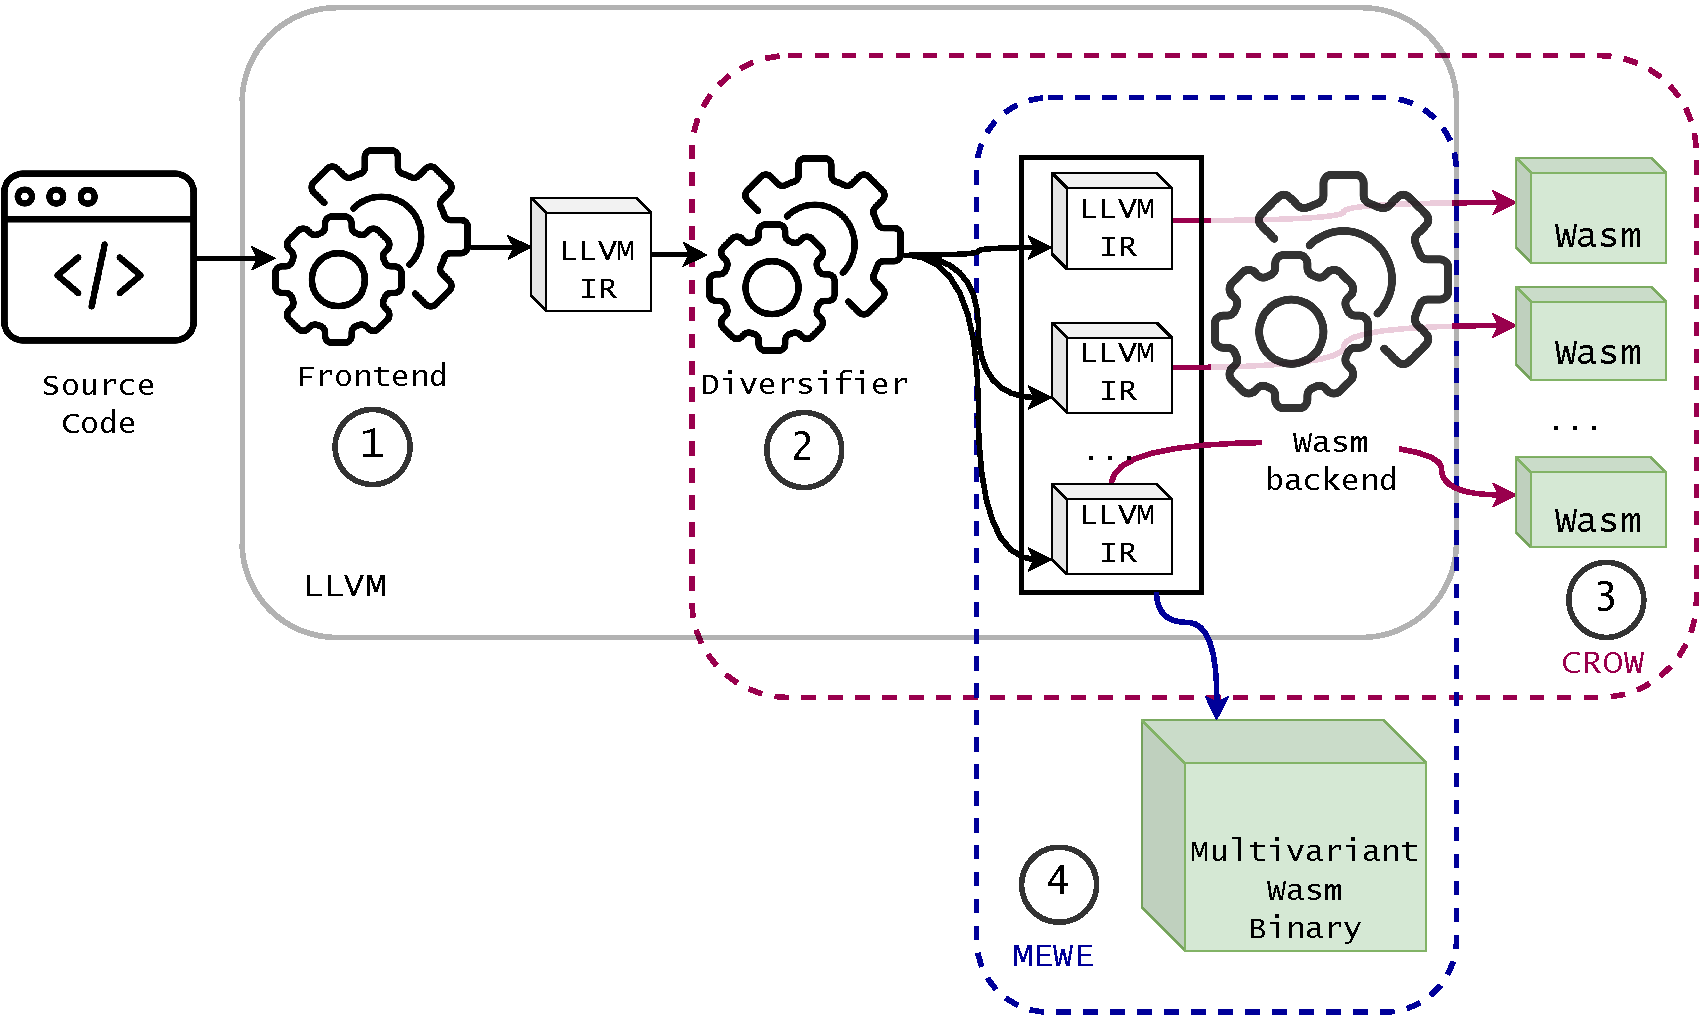
\includegraphics[width=\linewidth]{diagrams/architecture.pdf}
    \caption{Generic workflow to create \wasm program variants.}
    \label{diagrams:generic}
\end{figure*}


The global workflow in \autoref{diagrams:generic} starts by receiving source code. Then, the LLVM frontend transforms it into LLVM IR representation \step{1}. We alter the LLVM pipeline that compiles source code to Wasm, with the introduction of a Diversifier component.  
% Our diversifier and first contribution
The diversifier generates LLVM IR variants from of the output of the frontend \step{2}. 
The LLVM IR variants are inputs for our customized Wasm  backend. The Diversifier and the custom Wasm LLVM backend compose CROW, which creates \wasm program variants out of a source code program \step{3}. 
In addition, an orthogonal tool comes from the generation of LLVM IR variants at Step~\step{2}. MEWE  \cite{MEWE}, merges and creates multivariant binaries to provide MVE for \wasm \step{4}. 
%In \autoref{section:mewe} we describe MEWE in details.

%Our first technical contribution, CROW  \cite{CROW}, includes the implementation of the diversifier for LLVM and the customized \wasm backend. 


%Besides, as we discussed previously, our intention is also to study the impact of our contributions in edge computing and distributed systems and the top edge computing execution platforms, e.g. Cloudflare and Fastly, mostly take \wasm binaries as input. 
%LLVM, on the contrary, supports different languages, with a rich ecosystem of frontends it it can reliably be retargeted to \wasm, thanks to the corresponding mature component in the LLVM toolchain. In addition, the LLVM ecosystem as a whole is very active, providing us with many different tools to facilitate our research endeavour.
%In this chapter we summarize the technical details for our two contributions. \autoref{section:crow} we dissect the main components CROW \cite{CROW} implementation. Finally, in \autoref{section:mewe}, we describe the technical details of our second contribution, MEWE \cite{MEWE}.